\chapter{Negative Pion Cross Section Measurement}\label{ch:PionXS}
%{\raggedleft ``\emph{Y ella es flama que se eleva, Y es un p\'ajaro a volar.} \par}
%{\raggedleft \emph{En la noche que se incendia, estrella de oscuridad}\par}
%{\raggedleft \emph{que busca entre la tiniebla, la dulce hoguera del beso.}"\par}
%{\raggedleft -- Lila Downs, Benediction And Dream,  2002 -- \par}
%\vspace{0.5cm}

In this chapter, we show the result of the thin slice method to measure 
the ($\pi^-$-Ar) total hadronic cross section. In Section \ref{ch:PionXSRaw}, we start by measuring the raw cross section, i.e. the cross section obtained exclusively using data reconstruction, with no additional corrections. In Section \ref{ch:PionXSCorrections}, we apply a series of data manipulations geared toward the correction for the background contributions and thse correction for detection inefficiency, showing the final results in Section \ref{ch:FinalPion}.


\section{Raw Cross Section}\label{ch:PionXSRaw}
We measure the raw ($\pi^-$-Ar) total hadronic cross section as a function of the kinetic energy in the two chosen data sets, the -60A and -100A negative runs. 
As we will clarify in Section \ref{ch:PionXSCorrections},  the corrections to the raw cross section depend on the beam conditions and need to be calculated independently for the two datasets. Thus, we present here the measurement of the raw cross section on the two datasets separately.


As stated in section \ref{ch:XSRaw},  the raw cross section is given by the equation \label{eq:thinTargetXSSolved}
\begin{equation}
 \sigma_{TOT} (E_i)  = \frac{1}{n \delta X}\frac{N^{\text{TOT}}_{\text{Int}}(E_i)}{N^{\text{TOT}}_{\text{Inc}}(E_i)},
\end{equation}

where $N^{\text{TOT}}_{\text{Int}}$  is the measured number of particles interacting at kinetic energy $E_i$, $N^{\text{TOT}}_{\text{Inc}}$ is the  measured  number of particles incident  on an argon slice at  kinetic energy $E_i$,  $n$ is the density of the target centers  and $\delta X$ is the thickness of the argon slice. The density of the target centers and the slab thickness are $n = 0.021\cdot10^{24} \text{ cm}^{-3} $ and  $\delta X=0.47\text{ cm}$, respectively.


Figure \ref{fig:InteractingRaw} shows the distribution of  $N^{\text{TOT}}_{\text{Int}}$  as a function of the kinetic energy for the 60A dataset on the left and for the 100A dataset on the right. The data central points are represented by black dots, the statistical uncertainty is shown in black, while the systematic uncertainty is shown in red. Data is displayed over the $N^{\text{TOT}}_{\text{Int}}$  distribution obtained with a MC mixed sample of pions, muon and electrons (additional details on the composition will be provided in Section \ref{ch:BKGsubXS}). The contribution from the simulated pions is shown in blue, the one from secondaries in red, the one from muons in yellow and the ones from electrons in gray. 
The simulated pion's and backgrounds' contributions are stacked; the sum of the integrals from each particle species is normalized to the integral of the data.
 
Figure \ref{fig:IncidentRaw} shows the distribution of  $N^{\text{TOT}}_{\text{Inc}}$   for the 60A dataset on the left and for the 100A dataset on the right. Data is displayed over the MC. The same color scheme and normalization procedure is used for both the interacting and incident histograms. 


Figure \ref{fig:XSRaw} shows the raw cross section for the 60A dataset on the left and for the 100A dataset on the right, statistical uncertainty in black and systematic uncertainty in red. The raw data cross section is overlaid to the reconstructed cross section for the MC mixed sample, displayed in azure. Since the background contributions and the detector effects for the 60A and 100A sample are different, it is premature to compare the raw cross sections obtained from the two samples at this point.

We describe the calculation of the statistical uncertainty for the interacting, incident and cross section distributions in Section \ref{ch:StatUncertaintyXSRaw}; we describe the procedure to calculate the corresponding systematics uncertainty on Section \ref{ch:SysUncertaintyXSRaw}.

\begin{figure}[p]
\centering  
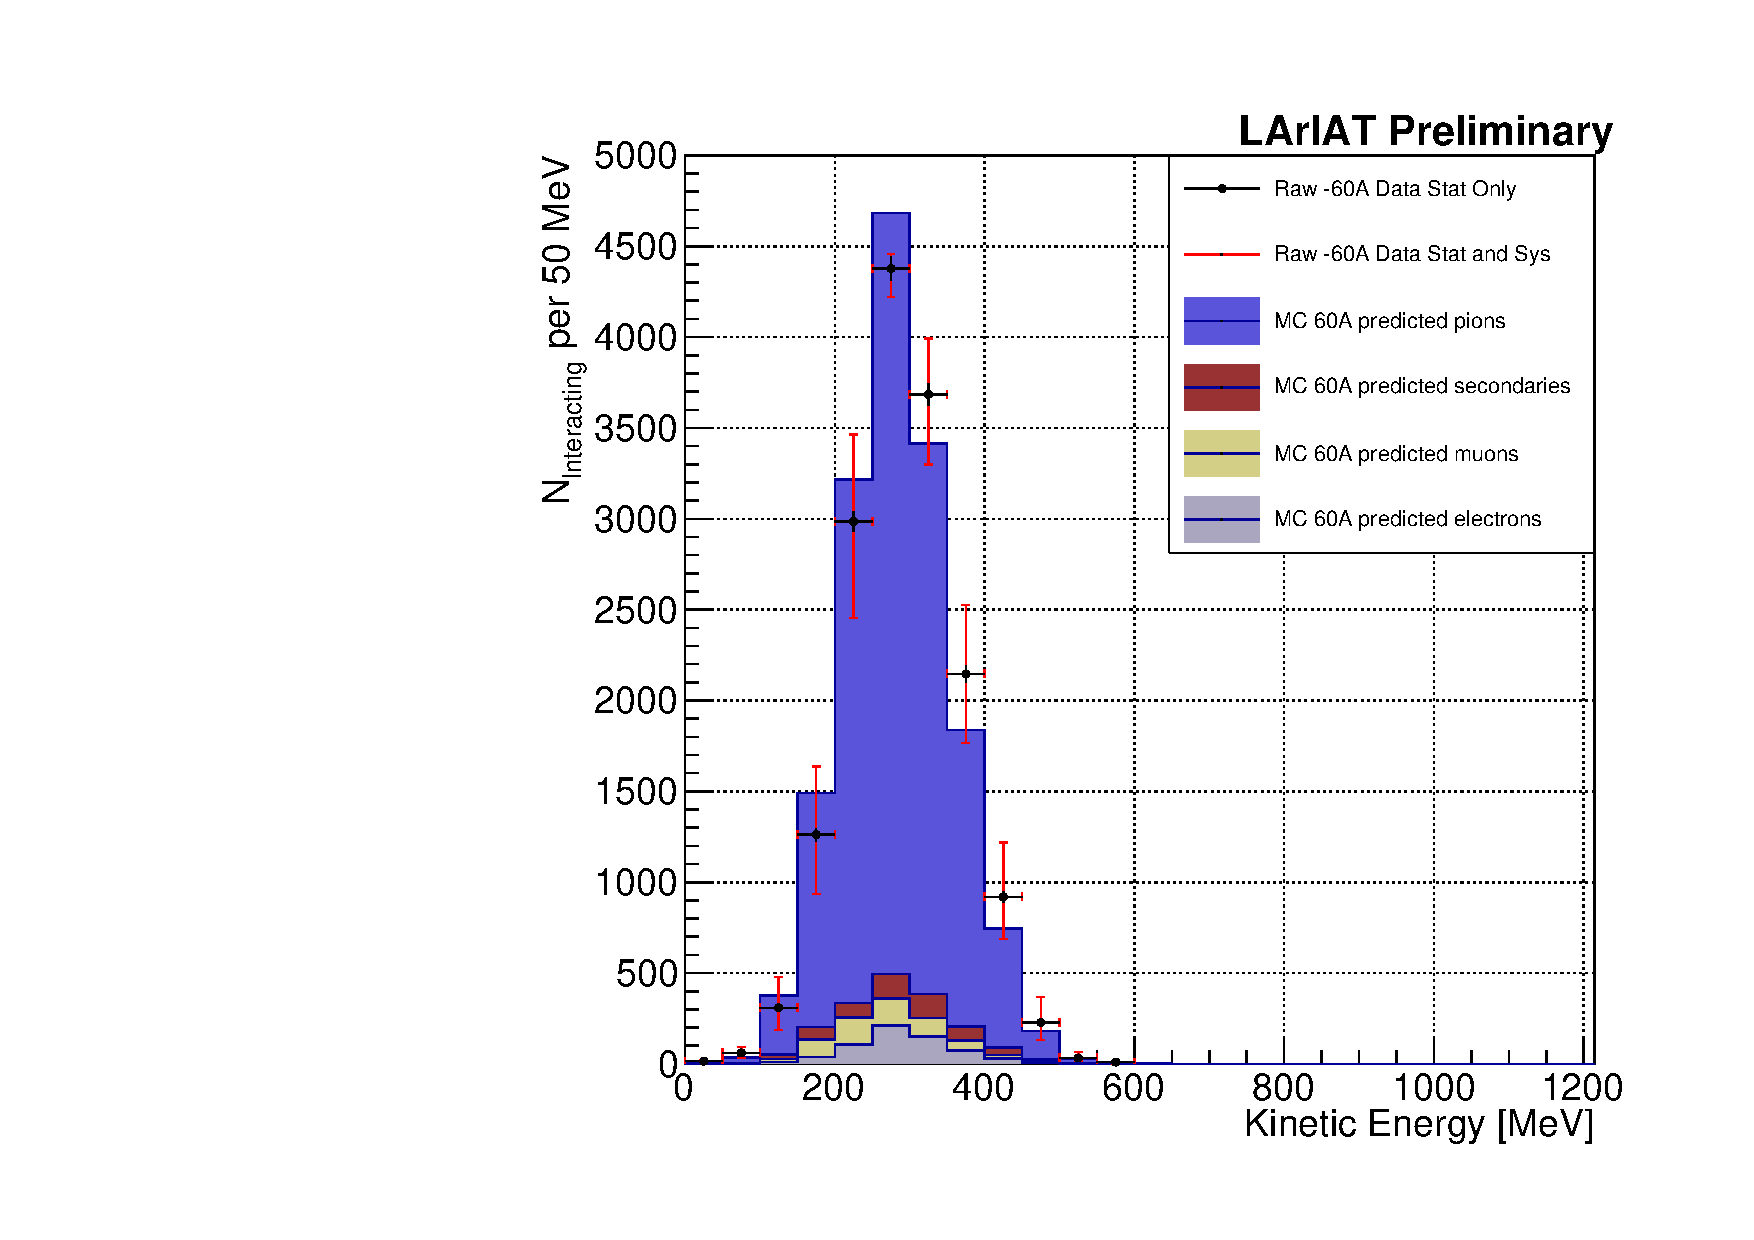
\includegraphics[width=0.48\textwidth]{Chapter-6/Images/Plots60A_MCData_Int_StatSyst.pdf}
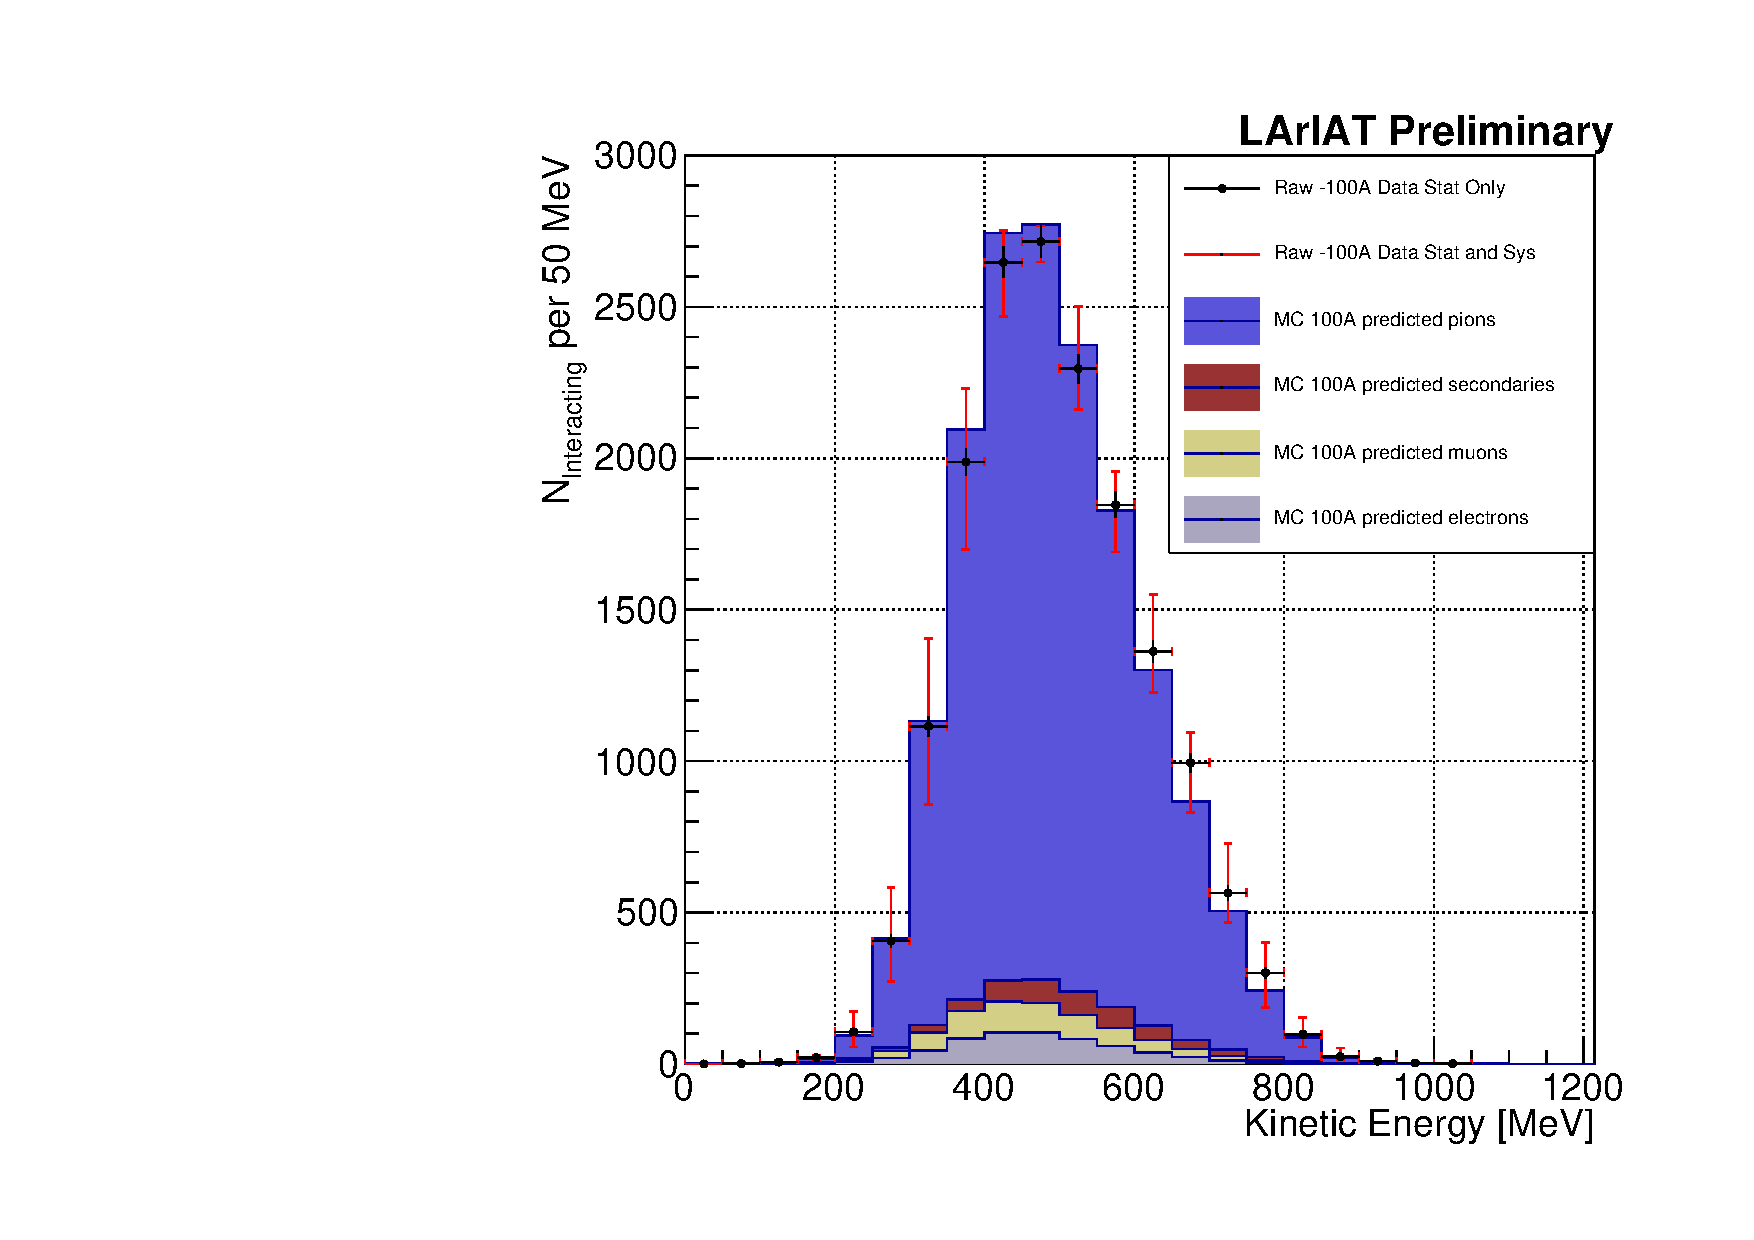
\includegraphics[width=0.48\textwidth]{Chapter-6/Images/Plots100A_MCData_Int_StatSyst.pdf}
\caption{Raw number of interacting pion candidates as a function of the reconstructed kinetic energy for the 60A runs (left) and for the 100A runs (right). The statistical uncertainties are shown in black, the systematic uncertainties in red.}
\label{fig:InteractingRaw}
\end{figure}


\begin{figure}
\centering  
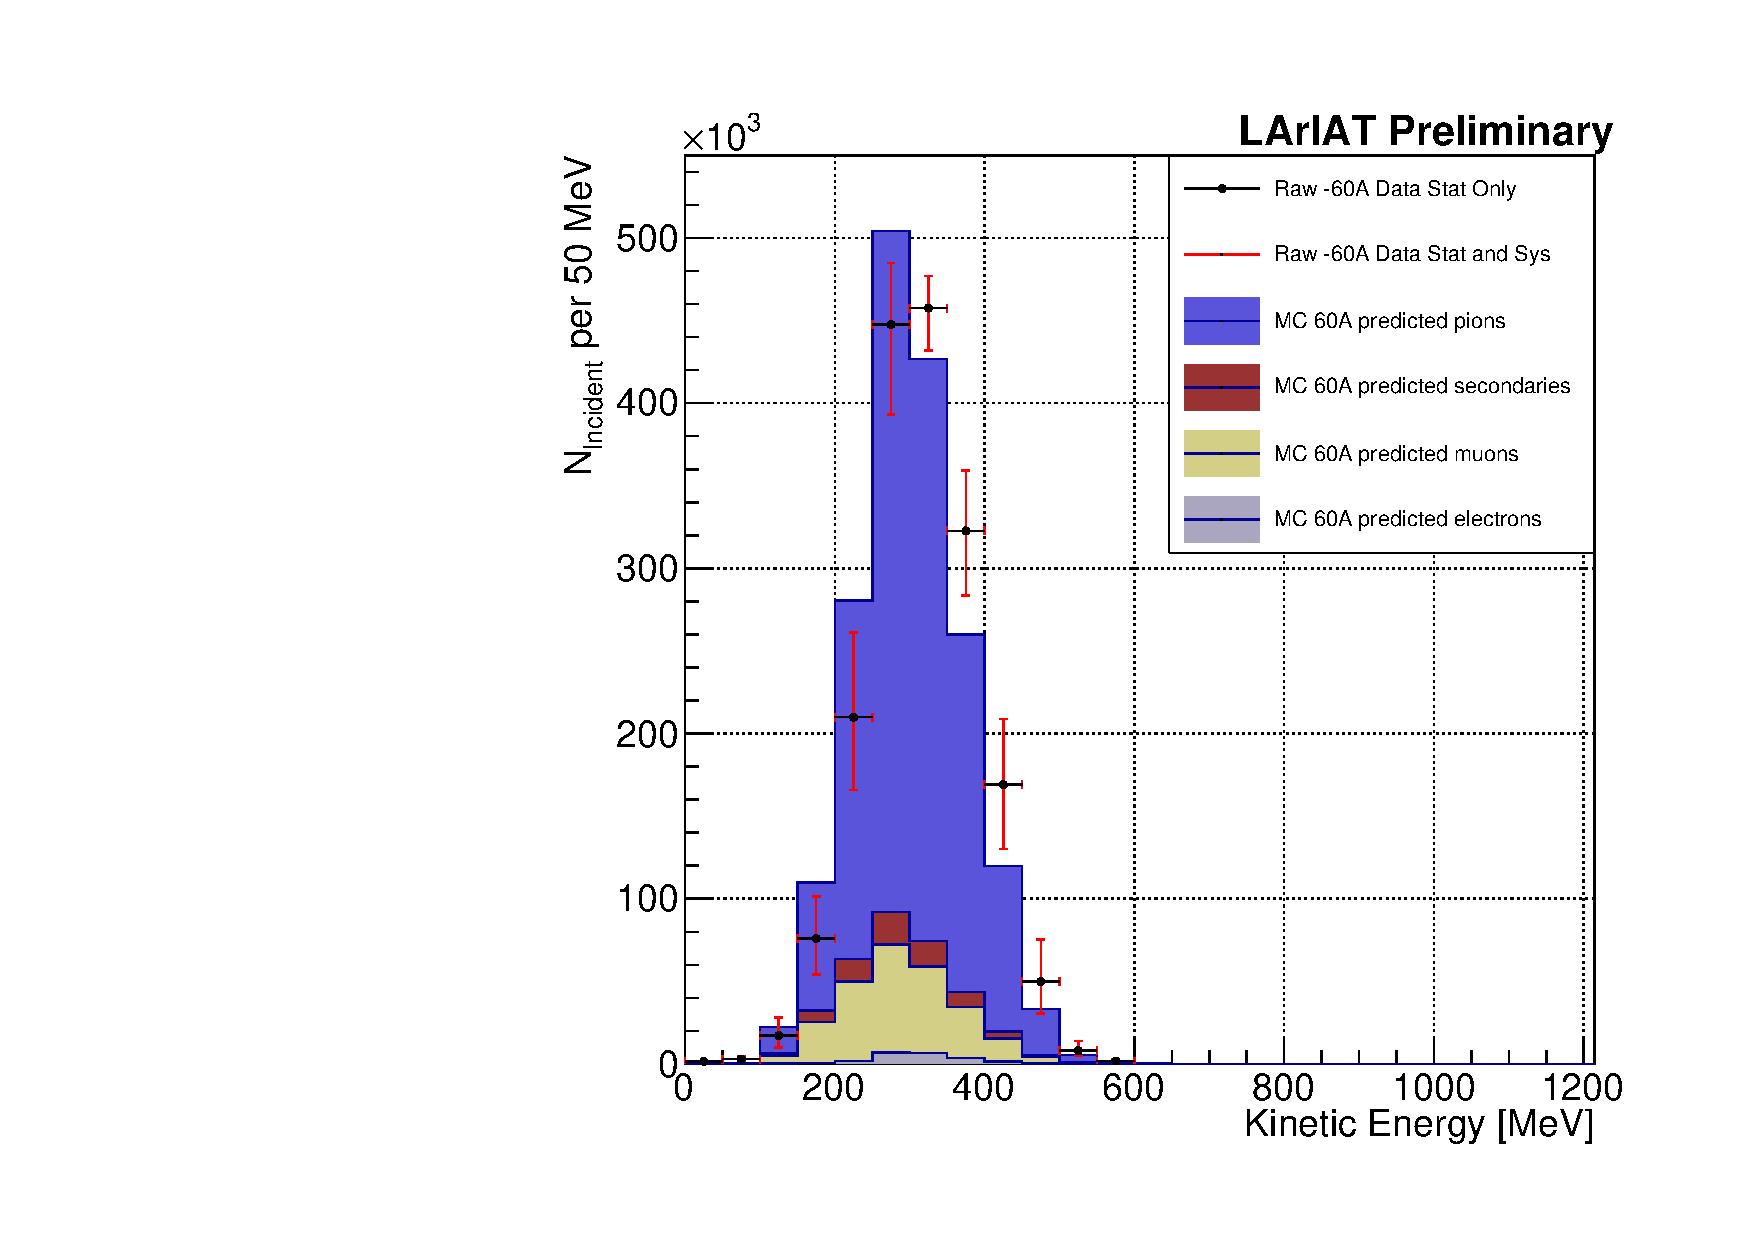
\includegraphics[width=0.48\textwidth]{Chapter-6/Images/Plots60A_MCData_Inc_StatSyst.pdf}
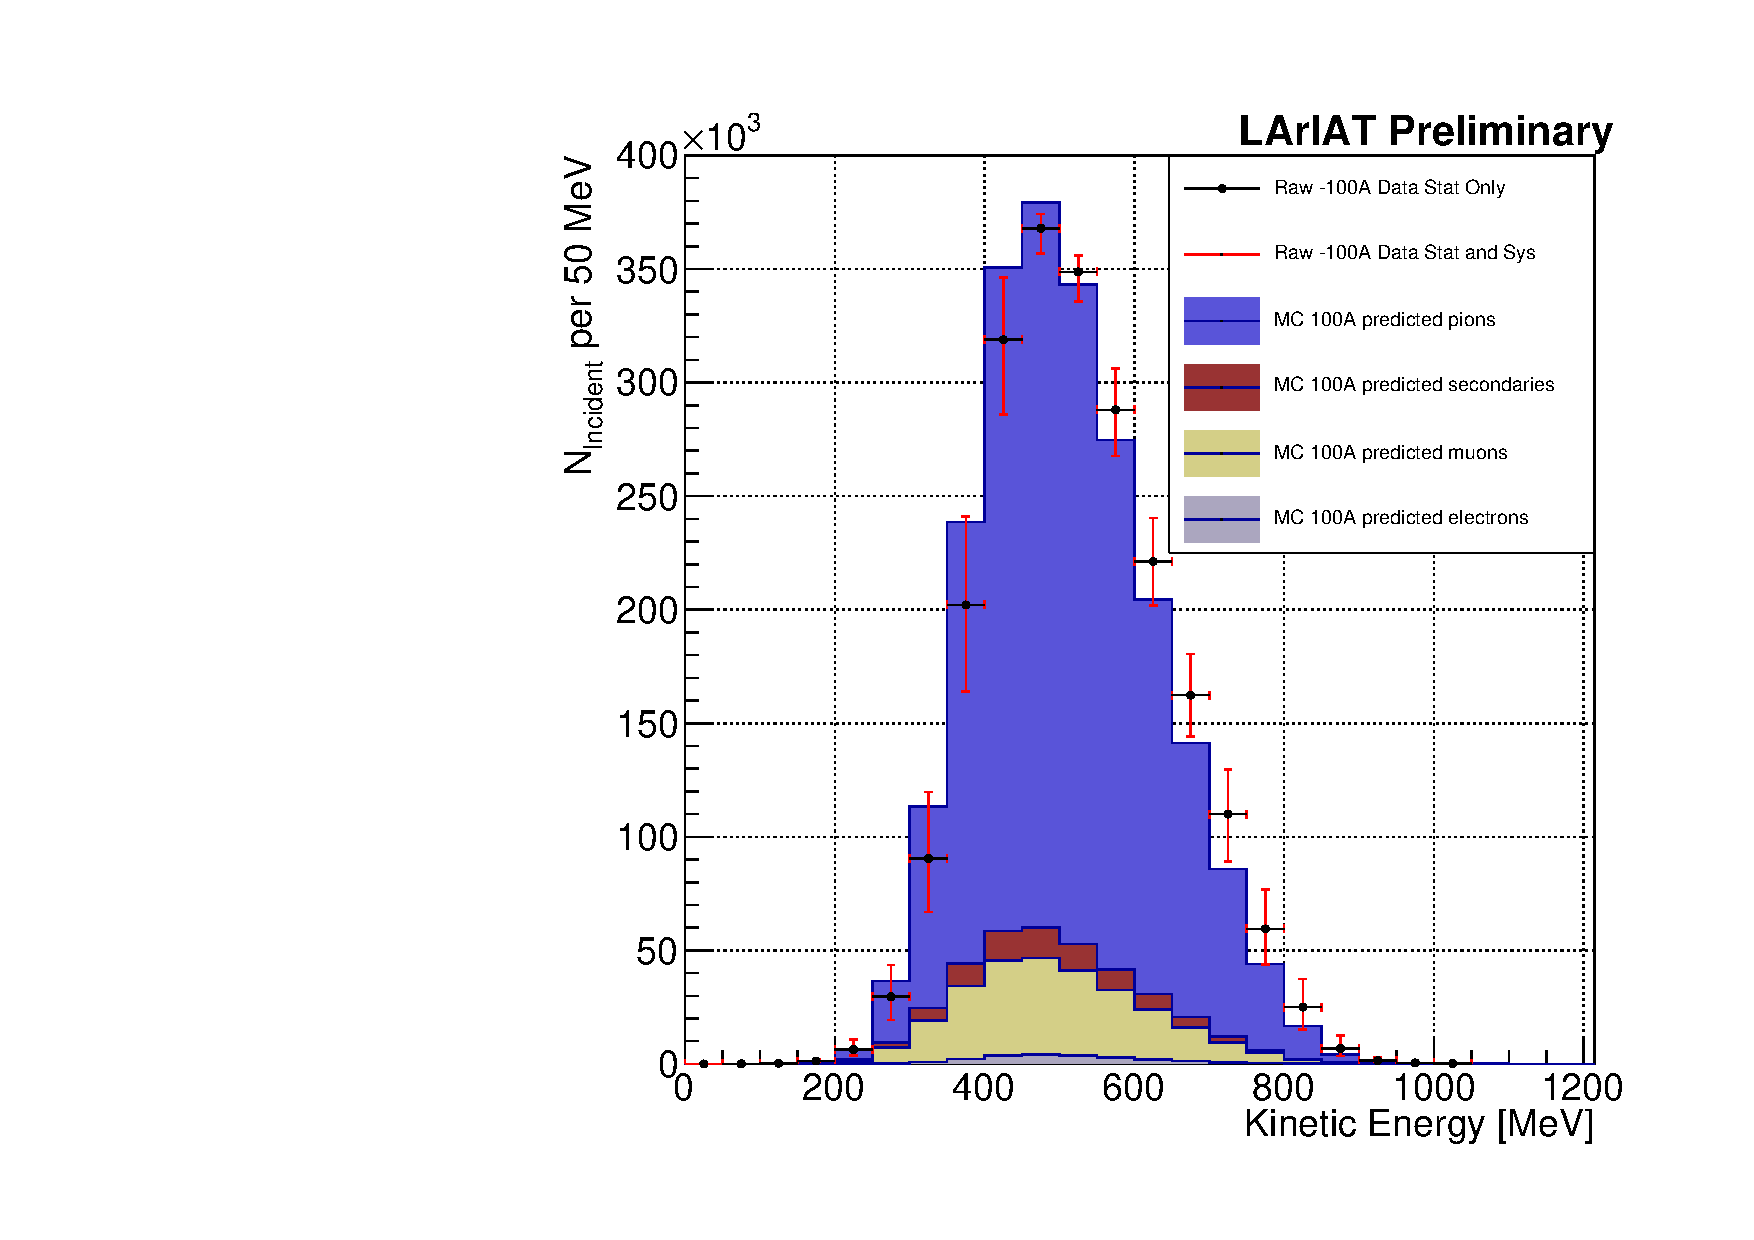
\includegraphics[width=0.48\textwidth]{Chapter-6/Images/Plots100A_MCData_Inc_StatSyst.pdf}
\caption{Raw number of incident pion candidates as a function of the reconstructed kinetic energy for the 60A runs (left) and for the 100A runs (right). The statistical uncertainty is shown in black, the systematic uncertainties in red.}
\label{fig:IncidentRaw}
\end{figure}

\begin{figure}
\centering  
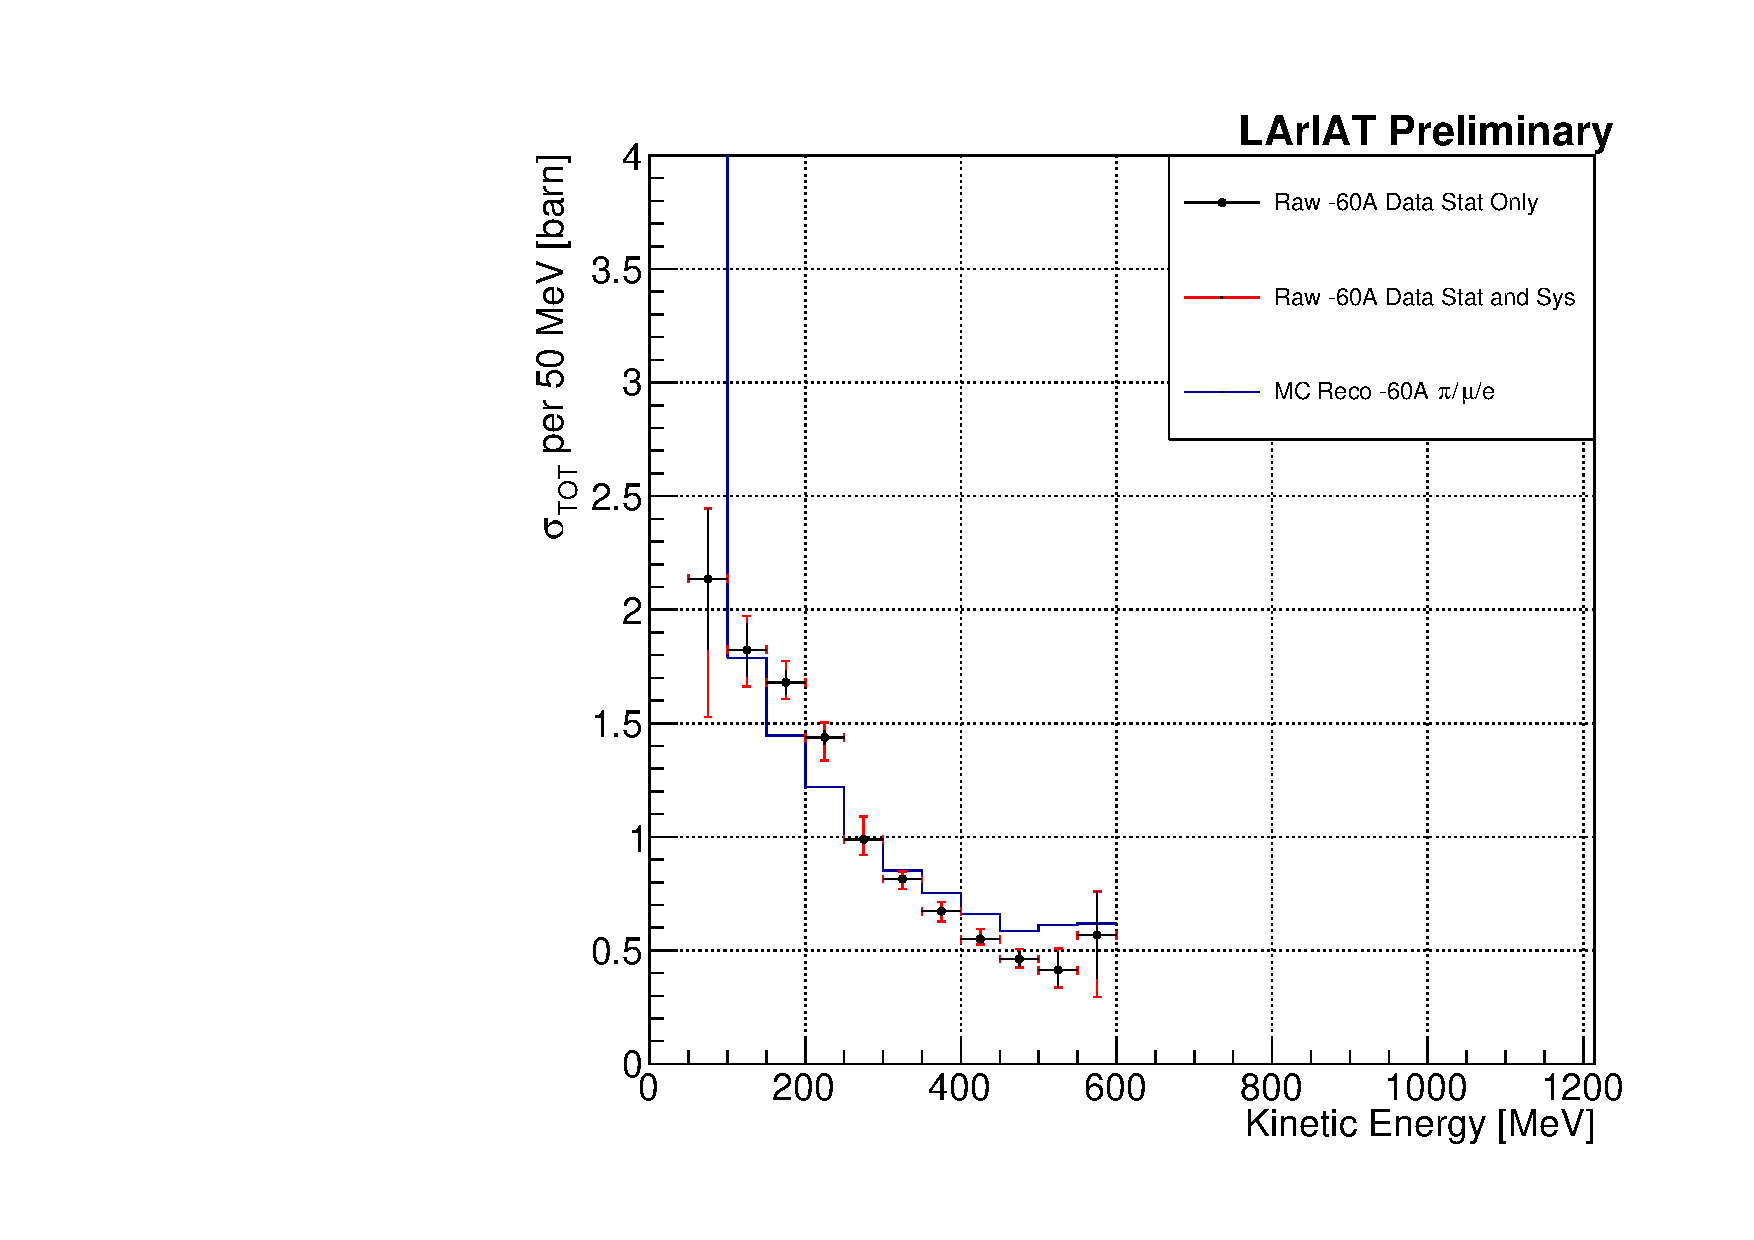
\includegraphics[width=0.48\textwidth]{Chapter-6/Images/Plots60A_MCData_XS_StatSyst.pdf}
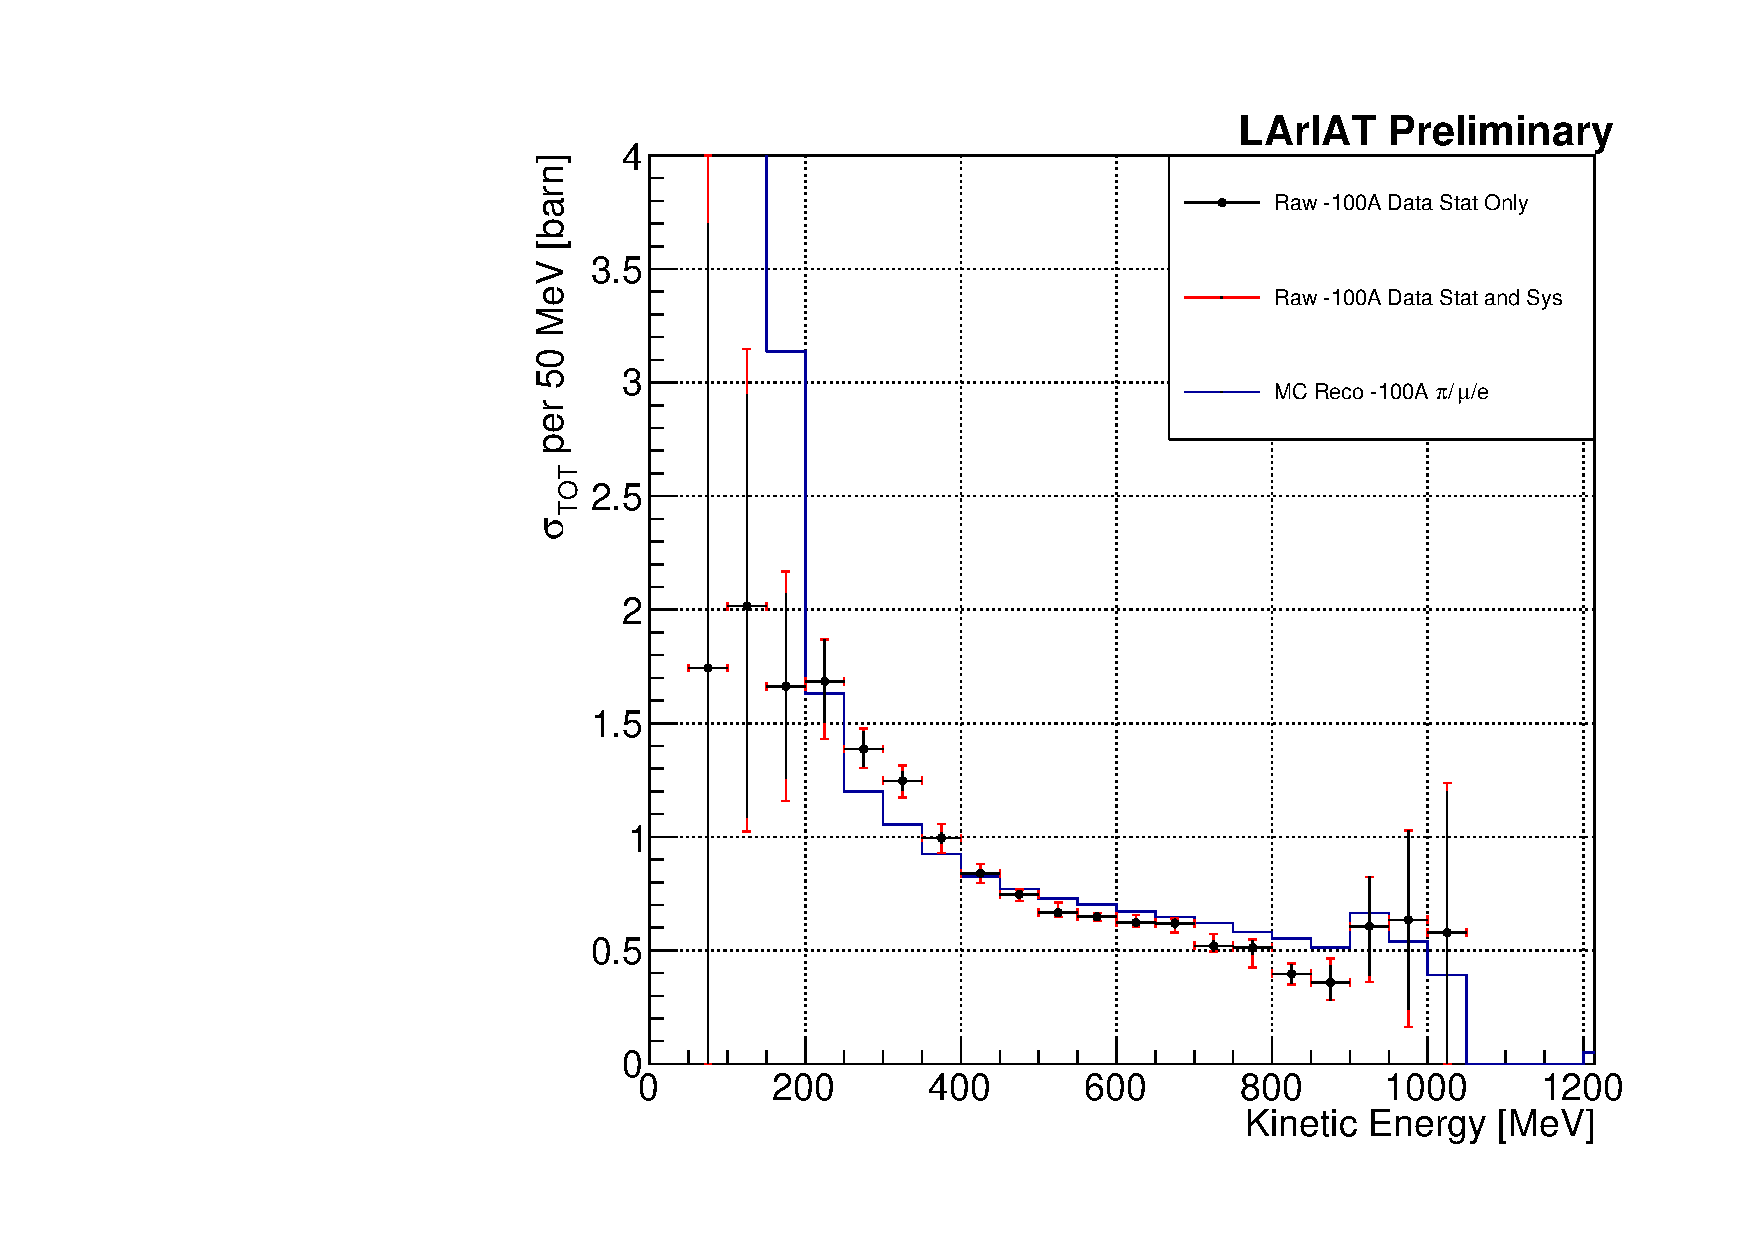
\includegraphics[width=0.48\textwidth]{Chapter-6/Images/Plots100A_MCData_XS_StatSyst.pdf}
\caption{Raw ($\pi^-$-Ar) total hadronic cross section for the 60A runs (left) and for the 100A runs (right). The statistical uncertainty is shown in black, the systematic uncertainties in red. The raw cross section obtained with a MC mixed sample of pions, muon and electrons in the percentage predicted by G4Beamline is shown in azure. }
\label{fig:XSRaw}
\end{figure}


\subsection{Statistical Uncertainty}\label{ch:StatUncertaintyXSRaw}
The statistical uncertainty for a given kinetic energy bin of the cross section  is calculated by error propagation from the statistical uncertainty on $N^{\text{TOT}}_{\text{Inc}}$ and $N^{\text{TOT}}_{\text{Int}}$ correspondent bin.  Since the number of incident particles in each energy bin is given by a simple counting, we assume that $N^{\text{TOT}}_{\text{Inc}}$ is distributed as a poissonian with mean and variance equal to $N^{\text{TOT}}_{\text{Inc}}$ in each bin.  
On the other hand, $N^{\text{TOT}}_{\text{Int}}$ follows a binomial distribution: a particle in a given energy bin might or might not interact.  The variance for the binomial is given by  
\begin{equation}
\text{\textsf{Var[}} N^{\text{TOT}}_{\text{Int}} \text{\textsf{]}}
 = \mathcal{N}P_{Interacting}(1-P_{Interacting}).
\label{eq:binVar}
\end{equation}

Since the interaction probability $P_{Interacting}$ is $\frac{ N^{\text{TOT}}_{\text{Int}}}{N^{\text{TOT}}_{\text{Inc}}}$ and the number of tries $\mathcal{N}$ is $N^{\text{TOT}}_{\text{Inc}}$, equation \ref{eq:binVar} translates into
\begin{equation}
\text{\textsf{Var[}} N^{\text{TOT}}_{\text{Int}} \text{\textsf{]}}
= N^{\text{TOT}}_{\text{Inc}}\frac{ N^{\text{TOT}}_{\text{Int}}}{N^{\text{TOT}}_{\text{Inc}}} (1-\frac{ N^{\text{TOT}}_{\text{Int}}}{N^{\text{TOT}}_{\text{Inc}}}) = N^{\text{TOT}}_{\text{Int}}(1-\frac{ N^{\text{TOT}}_{\text{Int}}}{N^{\text{TOT}}_{\text{Inc}}}). 
\end{equation}

$N^{\text{TOT}}_{\text{Inc}}$ and $N^{\text{TOT}}_{\text{Int}}$ are not independent.
The statistical uncertainty on the cross section is thus calculated as 
\begin{equation}
\delta\sigma_{TOT}(E) = \sigma_{TOT}(E) \Big(\frac{\delta N^{\text{TOT}}_{\text{Int}}}{N^{\text{TOT}}_{\text{Int}}}+\frac{\delta N^{\text{TOT}}_{\text{Inc}}}{N^{\text{TOT}}_{\text{Inc}}}\Big) 
\end{equation}
where:
\begin{eqnarray}
\delta N^{\text{TOT}}_{\text{Inc}} = \sqrt[]{N^{\text{TOT}}_{\text{Inc}}} \\
\delta N^{\text{TOT}}_{\text{Int}} = \sqrt[]{N^{\text{TOT}}_{\text{Int}}\Big(1-\frac{ N^{\text{TOT}}_{\text{Int}}}{N^{\text{TOT}}_{\text{Inc}}}\Big)}.
\end{eqnarray}



\subsection{Treatment of Systematics} \label{ch:SysUncertaintyXSRaw}
The only systematic effect considered in the measurement of the raw cross section results from the propagation of the uncertainty associate with the measurement of the kinetic energy at each argon slab. As shown in Section \ref{ch:kinEn}, the uncertainty on the kinetic energy of a pion candidate at the j$^{th}$ slab of argon  is given by

\begin{eqnarray}
\delta KE_{j} &=& \sqrt{\delta p_{Beam}^2 + \delta E_{Loss}^2 +  \delta  E_{\text{dep FF-j}}^2},\\
&=& \sqrt{(2\% \text{ }p_{Beam})^2 +  (\sim 7 \text{ [MeV]})^2 +  (j-1)^2 (\sim0.08\text{ [MeV]})^2}.
\end{eqnarray}

We propagate this uncertainty  by varying the energy measurement $KE_{j}$ at each argon slab. We calculating the $N^{\text{TOT}}_{\text{Inc}}$,  $N^{\text{TOT}}_{\text{Int}}$ and cross section plots in three cases: first assigning the measured $KE_{j}$ at each kinetic energy sampling, then assigning $KE_{j} + \delta KE_{j}$, and finally assigning $KE_{j} - \delta KE_{j}$. The difference between the values obtained using the $KE_{j}$ sampling and the maximum and minimum values in each kinetic energy bin determines the systematic uncertainty.

%We propagate this uncertainty  by calculating the $N^{\text{TOT}}_{\text{Inc}}$,  $N^{\text{TOT}}_{\text{Int}}$ and cross section plots twice: first assigning $KE_{j} + \delta KE_{j}$ at each kinetic energy sampling, then assigning $KE_{j} - \delta KE_{j}$. The difference between the central value and the maximum and minimum value in each kinetic energy bin gives the systematic uncertainty.

\section{Corrections to the Raw Cross Section}\label{ch:PionXSCorrections}
As described in section \ref{ch:MCCorrections} as series of corrections are needed to derive the true pion cross section from the raw cross section. 
These corrections are described in equation \ref{eq:C}, 

\begin{equation}
   \sigma^{\pi^-}_{TOT}(E_{i})  = \frac{1}{n \delta X}\frac{ \epsilon^{\text{Inc}}(E_i)  \hspace{0.2cm} C^{\pi MC}_{\text{Int}} (E_{i}) \hspace{0.2cm} N^{\text{TOT}}_{\text{Int}} (E_{i}) }{   \epsilon^{\text{Int}}(E_i) \hspace{0.2cm} C^{\pi MC}_{\text{Inc}} (E_{i}) \hspace{0.2cm}  N^{\text{TOT}}_{\text{Inc}} (E_{i})}.
 \tag{\ref{eq:C}}
\end{equation}



\subsection{Background subtraction}\label{ch:BKGsubXS}

\begin{figure}[htb]
\centering
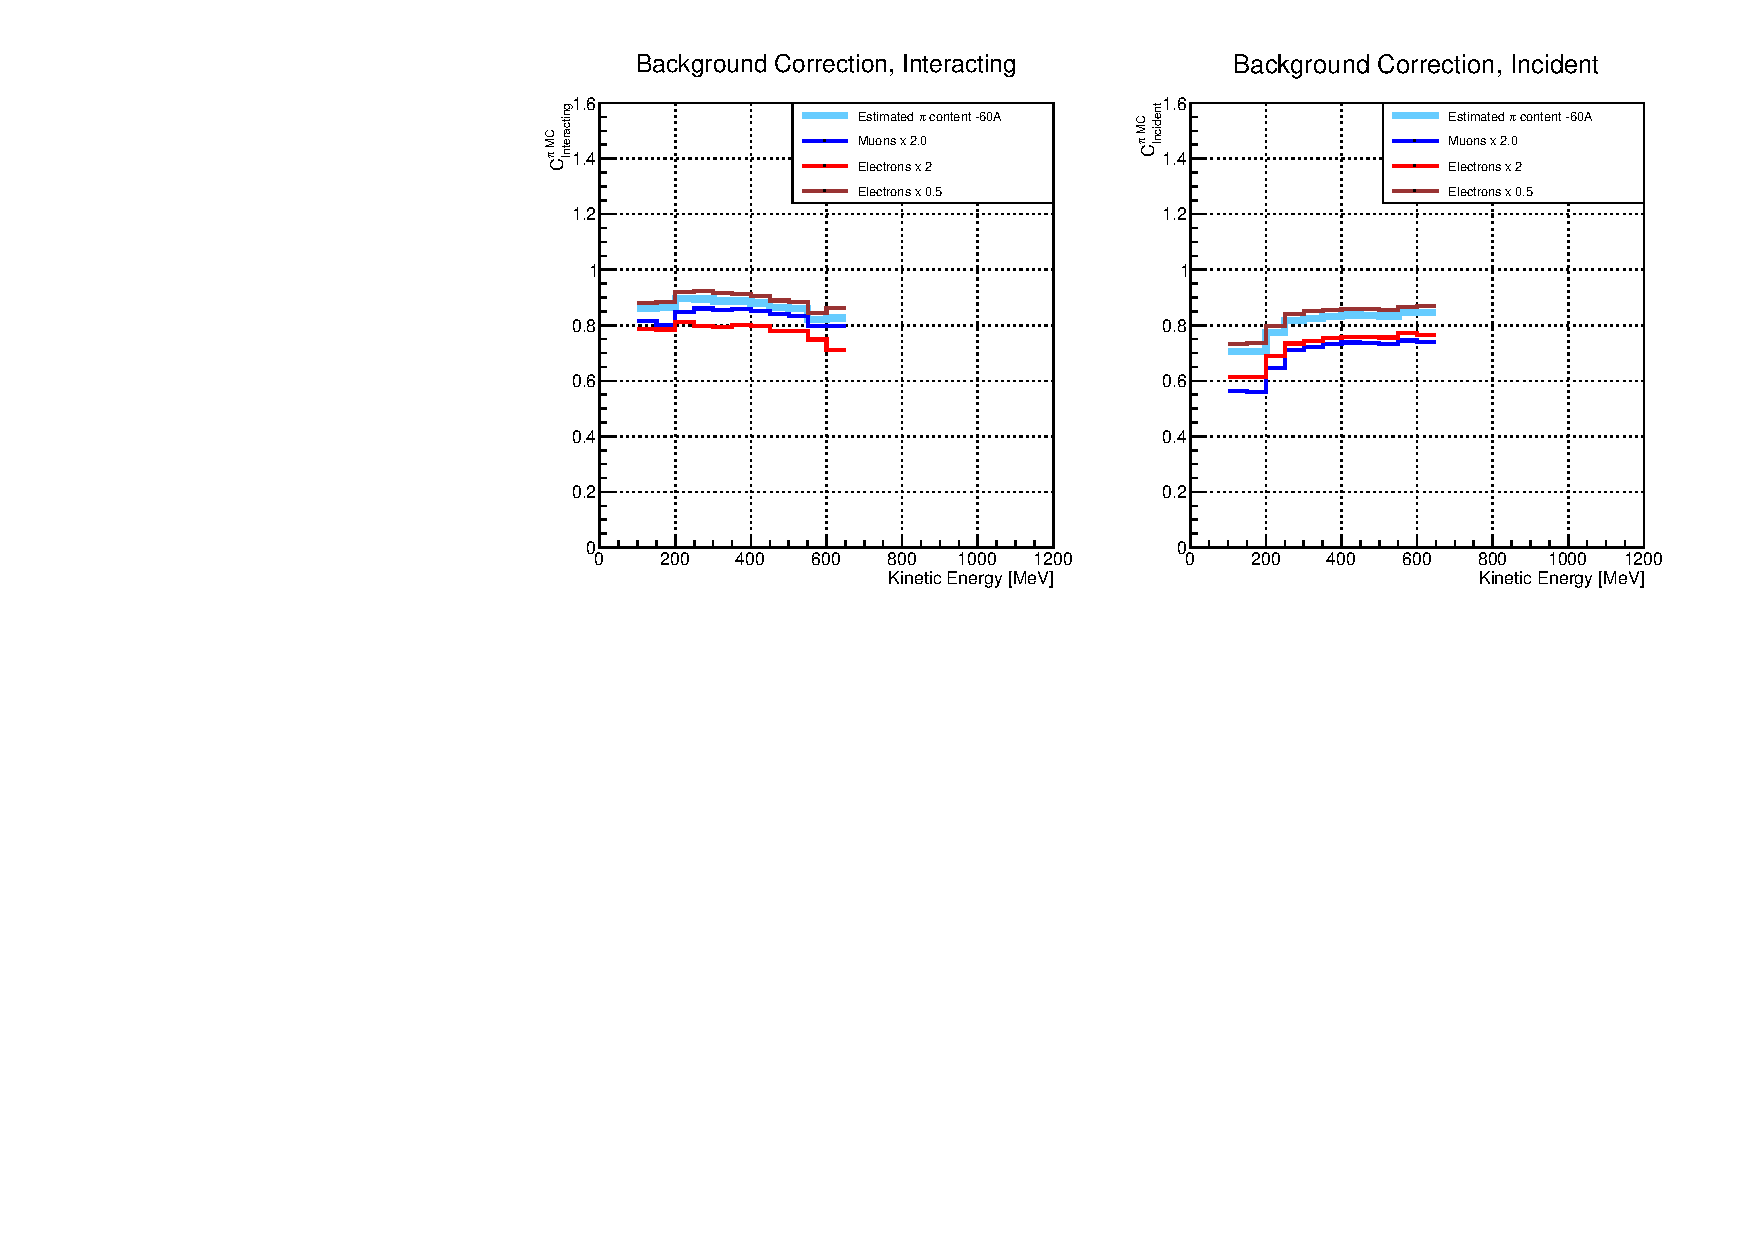
\includegraphics[width=\textwidth]{Chapter-6/Images/Bkg60A_inc_int.pdf}
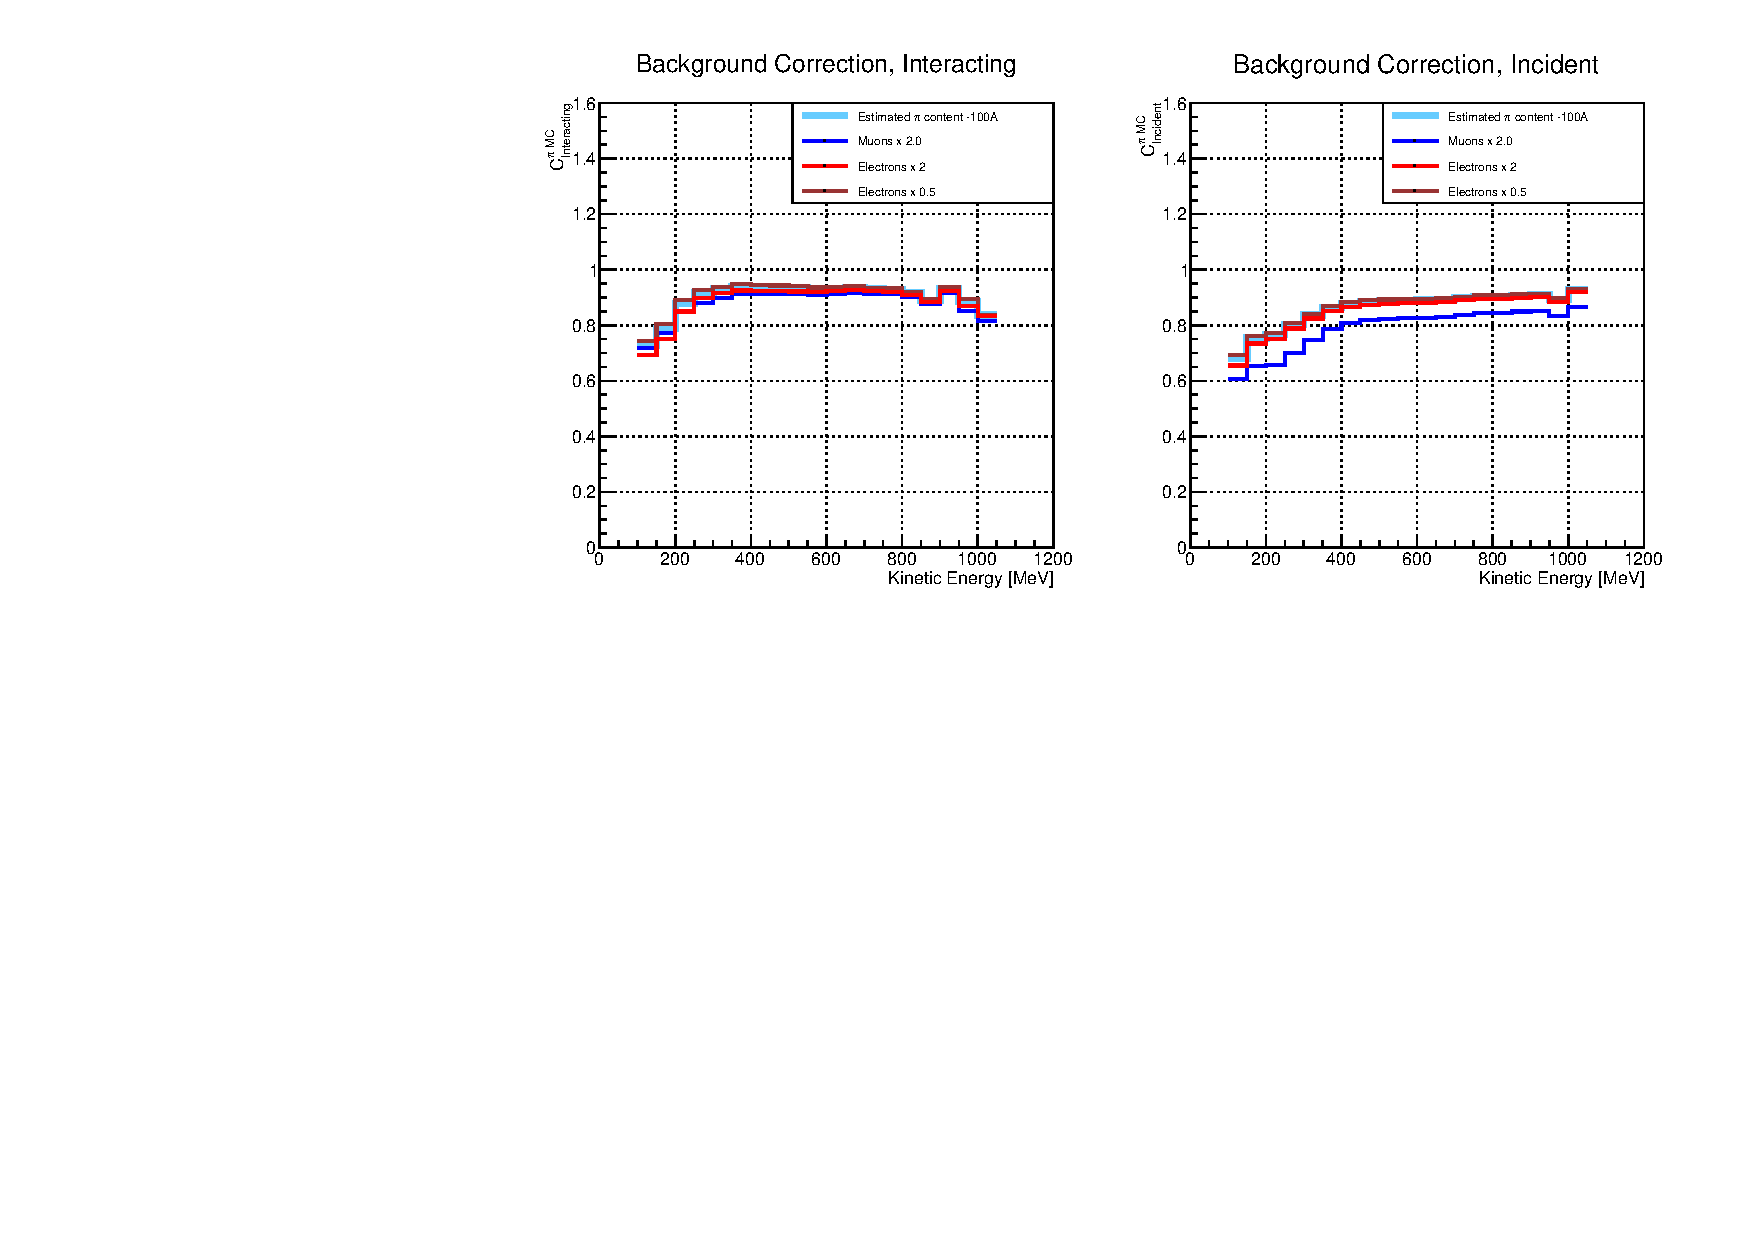
\includegraphics[width=\textwidth]{Chapter-6/Images/Bkg100A_inc_int.pdf}
\caption{.}
\label{fig:BkgCorr}
\end{figure}


\subsubsection{Treatment of Systematics}


\subsection{Efficiency Correction}
\subsubsection{Treatment of Systematics}


\section{Final Plots}\label{ch:FinalPion}

\begin{figure}[htb]
\centering
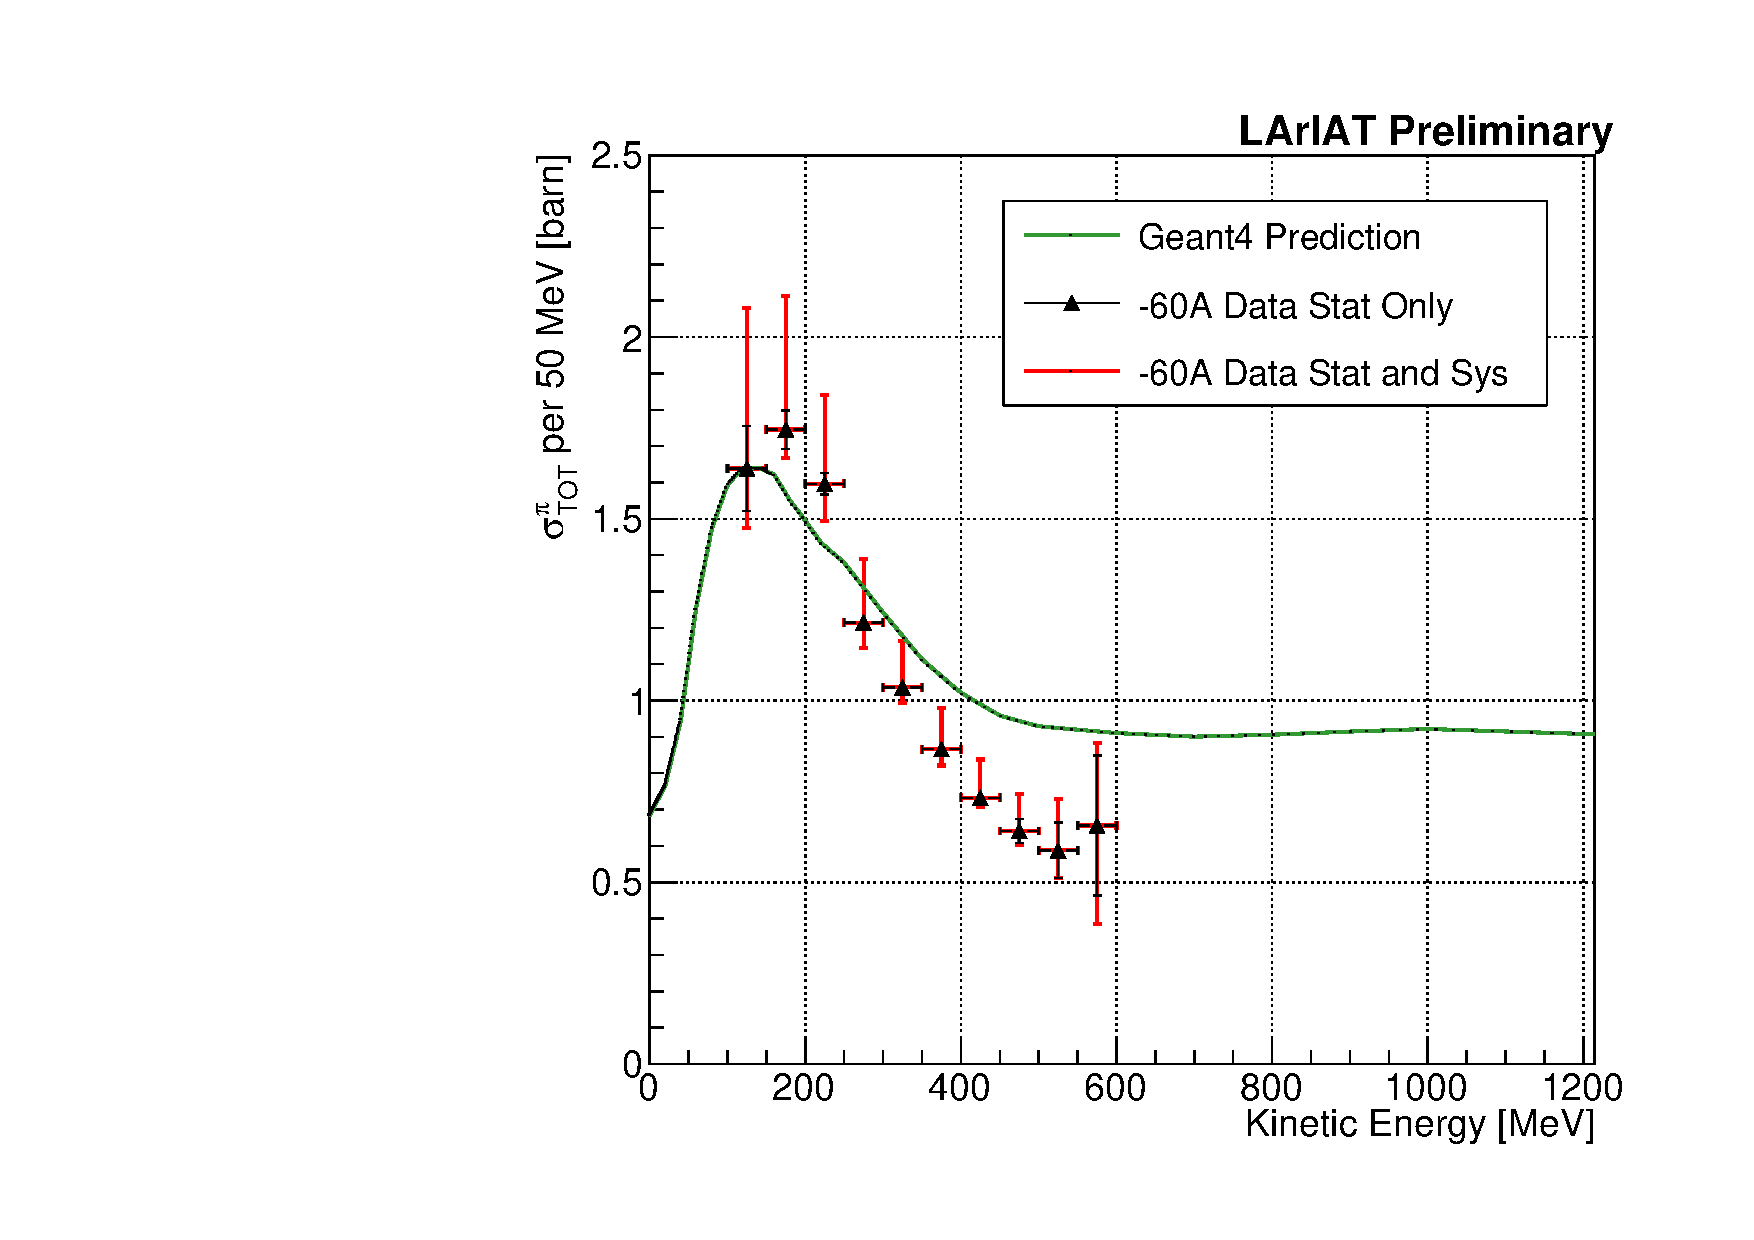
\includegraphics[width=0.48\textwidth]{Chapter-6/Images/TheMoneyPlot60A.pdf}
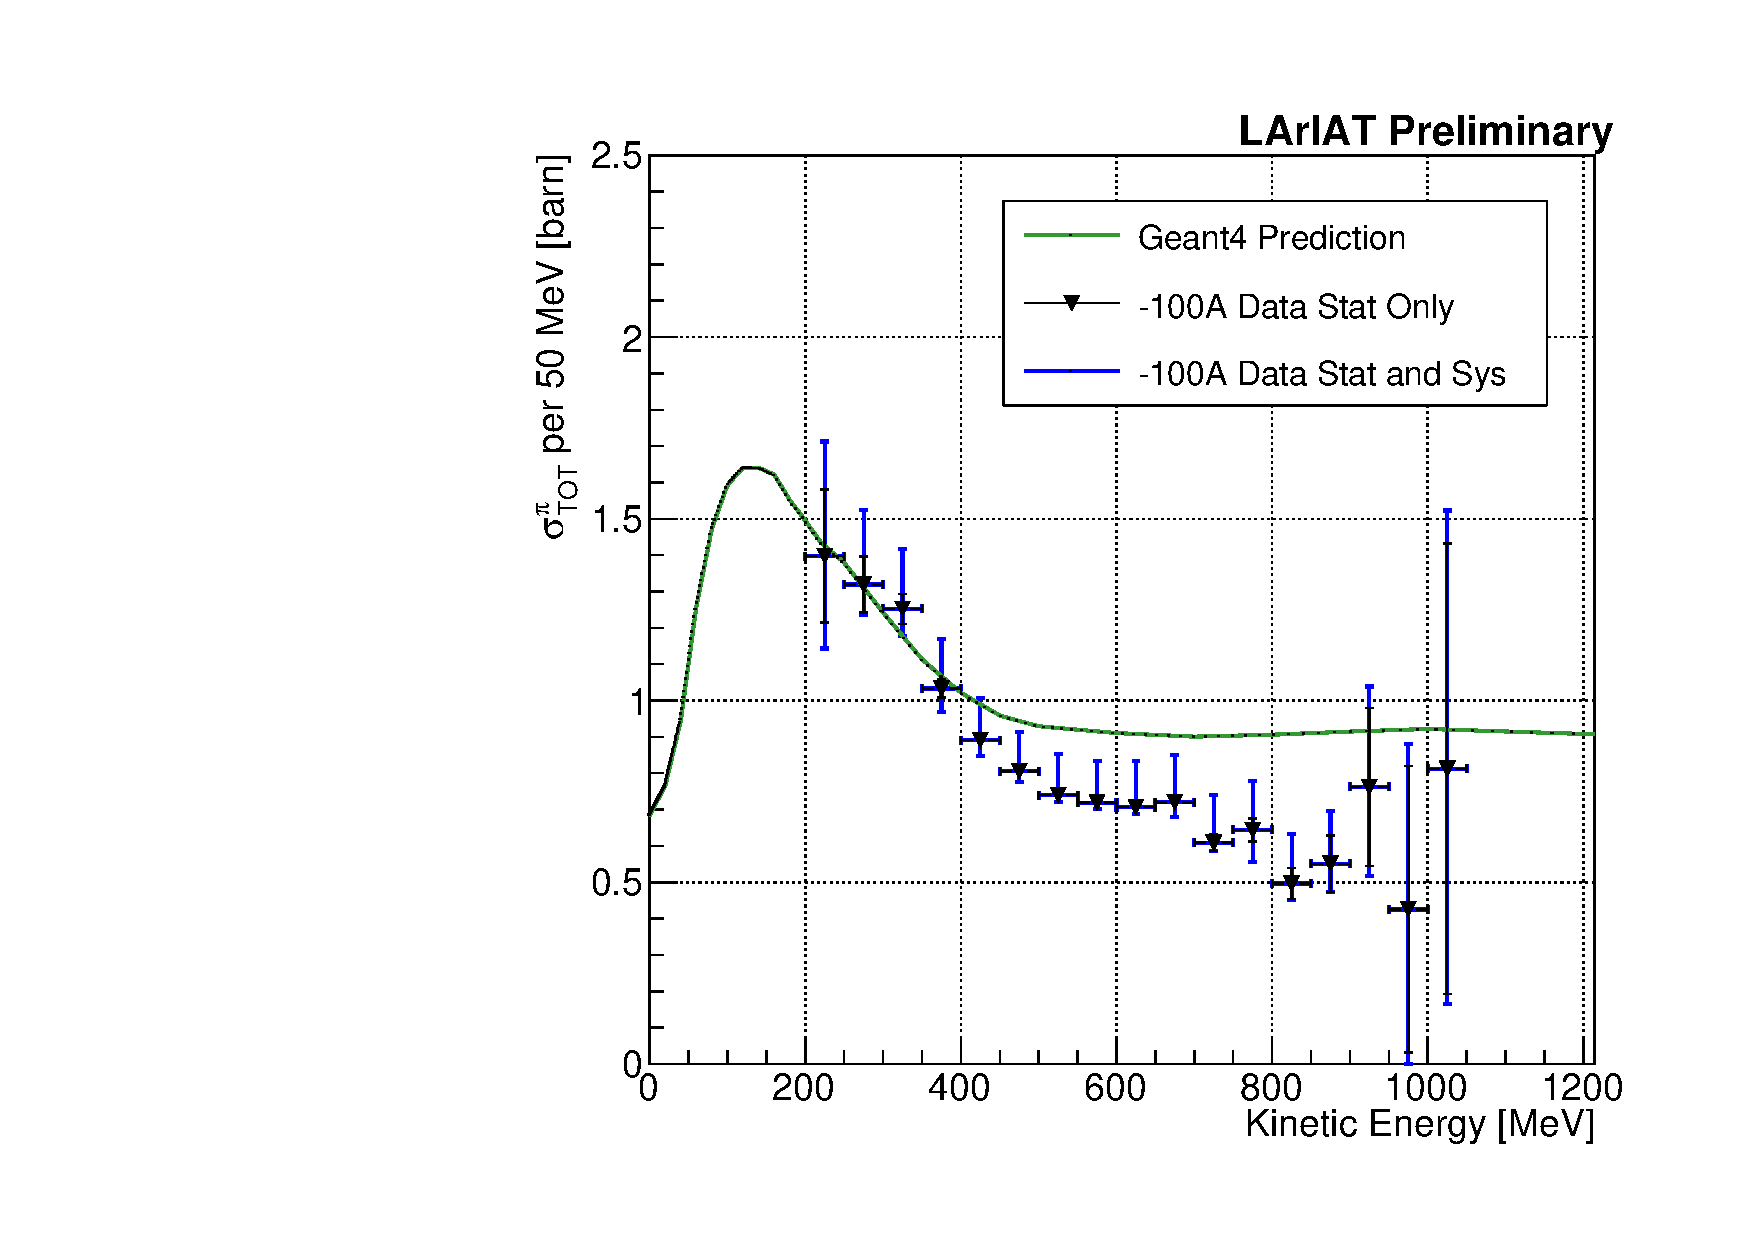
\includegraphics[width=0.48\textwidth]{Chapter-6/Images/TheMoneyPlot100A.pdf}
\caption{.}
\label{fig:FinalXSPion}
\end{figure}

\begin{figure}[htb]
\centering
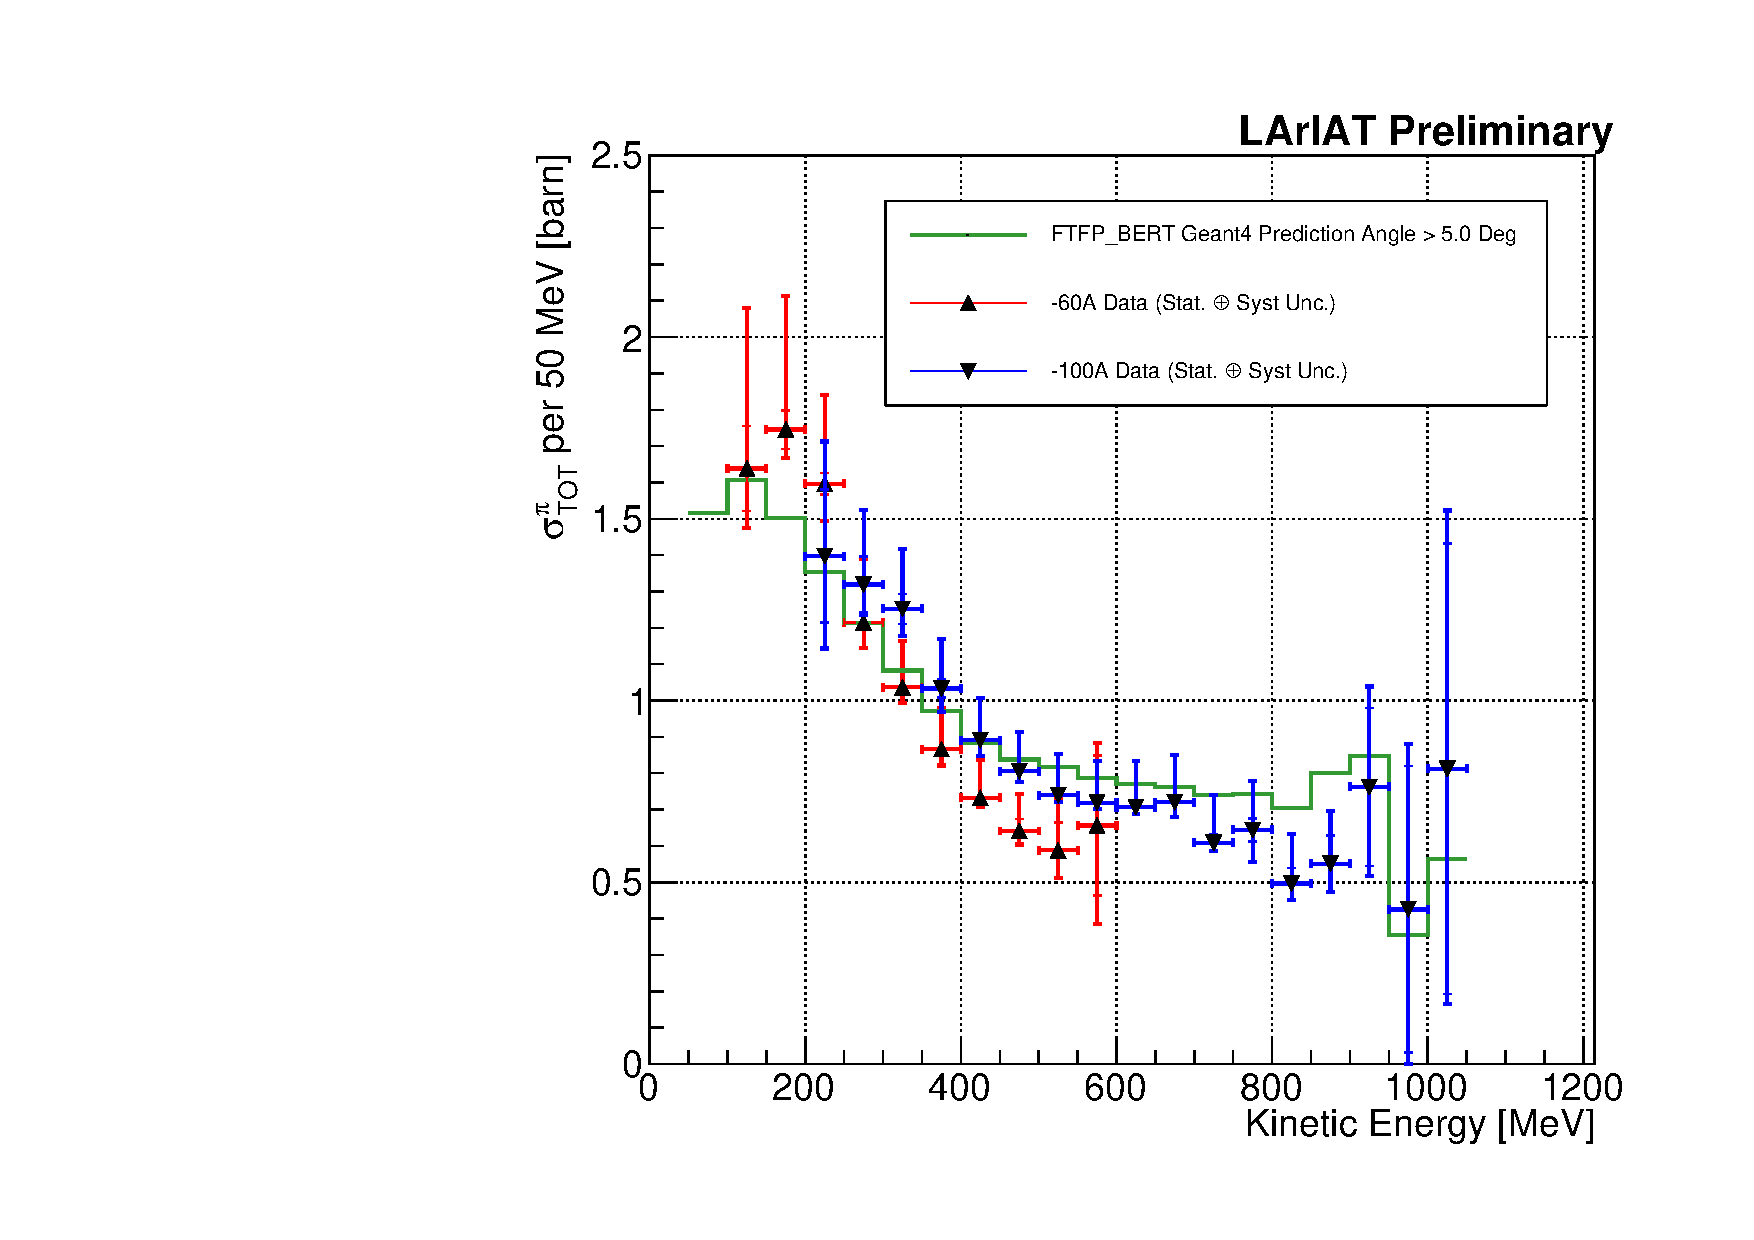
\includegraphics[width=0.48\textwidth]{Chapter-6/Images/TheMoneyPlot.pdf}
\caption{.}
\label{fig:FinalXSPion}
\end{figure}
